\documentclass[a4paper]{article}
\usepackage{babelbib}
\usepackage[dutch]{babel}
\usepackage{caption,tikz}
\captionsetup{width = 0.8\textwidth, font=small, textfont=it, labelfont=bf}
\usetikzlibrary{arrows.meta,positioning}
\usepackage[hidelinks,colorlinks=true,urlcolor=blue,linkcolor=,citecolor=]{hyperref}
\renewcommand{\subsectionautorefname}{Sectie}
\renewcommand{\figureautorefname}{Figuur}
\author{Benny Aalders \and Vincent Velthuizen}
\date{\today}
\title{Leeswijzer voor de map}
\hyphenation{programmeer-platform}
\newcounter{doen}
\renewcommand{\thedoen}{\textbf{\arabic{doen}.}}
\def\doen{\refstepcounter{doen}\thedoen}
\def\doenref#1{\ref{#1}}


\begin{document}
\maketitle
\begin{abstract}
\noindent
Bedankt voor uw deelname aan deze pretest! Als onderdeel van de pretest willen we natuurlijk graag uw feedback ontvangen. Daartoe hebben we een Google Form voor u klaar staan op \url{https://goo.gl/forms/Wo8pnnZHwI3MsmLV2}. Vul eerst de eerste twee pagina's met vragen in voor u verder gaat met dit document. De derde (laatste) pagina vult u in nadat u het materiaal heeft bekeken.
\end{abstract}
\renewcommand{\refname}{\vspace{-2em}}
\noindent De volgende bestanden horen bij de pretest:
\bibliographystyle{babunsrt-fl} 
  \bibliography{alle-bestanden}
We beschrijven hier met welk doel de bestanden gemaakt zijn en hoe u ze het best kunt lezen.

\section{Introductie: Computational Thinking tijdens de wiskundelessen}
Bij wiskunde ontwikkelen leerlingen op een natuurlijke manier vaardigheden die helpen de leerdoelen van Computational Thinking te verwezelijken. In opdracht van SLO hebben wij gezocht naar manieren om Computational-Thinking-leerdoelen expliciet te verwezenlijken tijdens de wiskundelessen, zonder dat het wiskundecurriculum  moet worden aangepast. Voor meer informatie over Computational Thinking verwijzen we door naar \href{http://curriculumvandetoekomst.slo.nl/21e-eeuwse-vaardigheden/digitale-geletterdheid/computational-thinking}{curriculumvandetoekomst.slo.nl}\footnote{Exacte URL: \url{http://curriculumvandetoekomst.slo.nl/21e-eeuwse-vaardigheden/digitale-geletterdheid/computational-thinking}}.

Onze oplossing is gebaseerd  op het volgende idee:
\begin{center}\bfseries\noindent Door leerlingen (wiskundige) problemen te laten programmeren, wordt het merendeel van de leerdoelen Computational Thinking gehaald en het begrip van de (wiskundige) oplossingen vergroot.
\end{center}
We willen de leerlingen daarom programma's laten schrijven, gebaseerd op de lesstof wiskunde. Dit doen ze na de reguliere oefening met de stof, hierdoor kunnen ze hun eigen antwoorden gebruiken bij het valideren van hun programma's (en vice versa).

Om een programma te schrijven dat kan helpen bij een bepaald wiskundeonderwerp, moet een leerling vijf stappen doorlopen. \hfill\\
\doenref{lesboek} Het lesboek op de gebruikelijke manier doorlopen. De theorie en technieken horend bij een bepaald onderwerp worden behandeld en de leerling gaat aan de slag met zijn opgaven.

Op een zeker moment herkent en onderkent de leerling de repetitieve aard van zijn bezigheden. \hfill\\
\doenref{geschikt} De leerling moet bedenken of een computerprogramma hem kan helpen bij de opdrachten. \hfill\\
\doenref{verwoorden} Om hier goed antwoord op te kunnen geven, moet de leerling nadenken over de verwoording van het probleem. Beter gezegd: Kan ik dit probleem zodanig verwoorden dat een computer het kan ``begrijpen''. Met andere worden formuleer het algoritme (bijvoorbeeld geschreven in ``pseudocode''). \hfill\\
\doenref{implementeer} Daarna moet de leerling het algoritme implementeren.\hfill\\
\doenref{controleer} Tot slot moet de leerling zijn of haar programma controleren. Dit kan alleen als hij weet wat de juiste uitvoer van zijn programma moet zijn. Dit waarborgt dat een leerling nog steeds leert om de sommen met de hand uit te rekenen. 

De leerling heeft nu een werkend programma dat hij kan en mag gebruiken wanneer het hem belieft en wanneer de docent dit toestaat. De docent heeft hierover de controle (in \autoref{programmeerplatform} komen we hier op terug). In \autoref{schema} hebben we dit samengevat.

Extra aandacht verdienen stap \ref{geschikt} en \ref{verwoorden} Ten eerste zijn deze stappen niet los van elkaar te zien. Immers, het antwoord op de vraag van \ref{verwoorden} bepaalt het antwoordt op de vraag van \ref{geschikt} Daarnaast zou het antwoord op vraag \ref{geschikt} ook prima ``nee'' kunnen zijn. Dit is geen probleem. Het is zelfs goed: Computational Thinking betekent niet dat leerlingen alles door een computer moeten laten doen. Ze moeten ook kunnen bedenken dat een programma schrijven niet altijd even makkelijk en/of nuttig is. 
\begin{figure}[ht!]\centering
\makebox[\textwidth][c]{
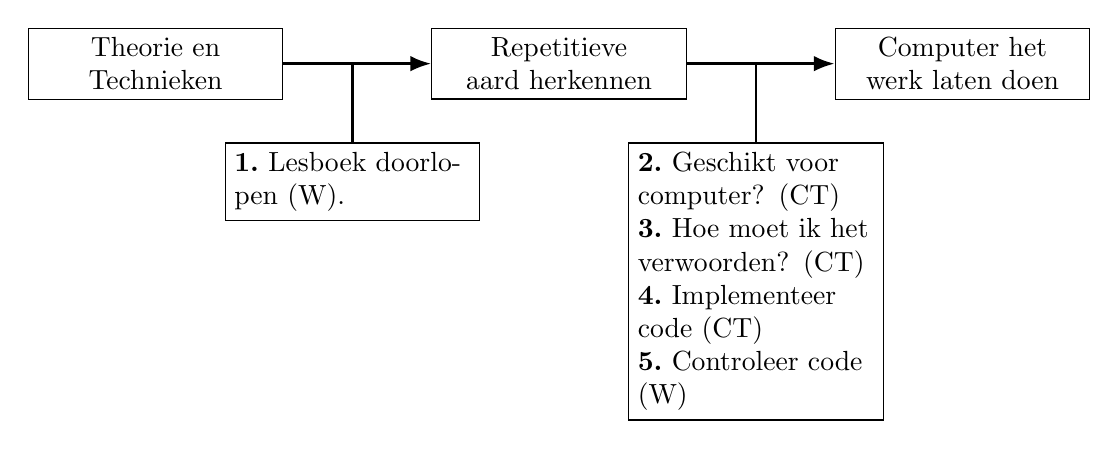
\begin{tikzpicture}[>=Latex, every node/.style={text width=3cm}]
	\begin{scope}[every node/.style={align=center, text width=3cm}]
		\node [draw] (theorie) 
			{Theorie en Technieken};
				\node [right=of theorie.center, inner sep=0pt, line width=0pt] (dummie1) {};
		\node [draw, right=of dummie1.center] (rep) 
			{Repetitieve aard herkennen};
				\node [right=of rep.center, inner sep=0pt, line width=0pt] (dummie2) {};
		\node [draw, right=of dummie2.center] (schrijven) 
			{Computer het werk  laten doen};
	\end{scope}
	\node [draw, below =of dummie1.center)] (doorlopen) 
		{\doen\ Lesboek doorlopen (W).\label{lesboek}};
	\node [draw, below=of dummie2.center] (vragen)
		{\doen\ Geschikt voor computer? (CT)\label{geschikt}\\
		  \doen\ Hoe moet ik het verwoorden? (CT)\label{verwoorden}\\
		  \doen\ Implementeer code (CT)\label{implementeer}\\
		  \doen\ Controleer code (W)\label{controleer}};
	\begin{scope}[line width=1pt]
		\draw [->] (theorie) to (rep);
		\draw [->] (rep) to (schrijven);
		\draw (dummie1) to (doorlopen);
		\draw (dummie2) to (vragen);
	\end{scope}
\end{tikzpicture}
}
\caption{Een schematische weergave van het proces dat een leerling moet doorlopen om een programma te schrijven bij de theorie. (W) geeft aan dat een leerling wiskundevaardigheden nodig heeft voor een goed resultaat. (CT) doet dat voor Computational Thinking.\label{schema}}
\end{figure}

\section{De bestanden}
De bestanden \cite{voorwoord,opdrachten,instructies} zijn  geschreven om een beeld te schetsen van een implementatie van onze methode, zoals wij die voor ogen hebben. In \cite{progplatform} is te lezen hoe goed de producten van de drie grootste producenten van grafische rekenmachines aansluiten bij onze methode.


\subsection{Voorbeeld van een voorwoord \cite{voorwoord}} Voor de implementatie van onze methode is nieuw materiaal nodig. Materiaal wat aansluit op het bestaande wiskundeprogramma. In \cite{voorwoord} is een voorwoord te lezen van zulk materiaal. Aan de hand van dit voorwoord moet een docent/vakgroep/school kunnen besluiten of ze dit materiaal gaan gebruiken.  We raden aan om dit bestand eerst te lezen.

We vragen u zich in te beelden dat een wiskundedocent de boeken van Getal \& Ruimte gebruikt voor zijn/haar lessen. Het voorwoord en de materialen zijn daar op geschreven. Voor de andere wiskunde methoden zouden ook andere (op dezelfde of vergelijkbare stof gebaseerde) Computational Thinking methode moeten worden gemaakt.

\subsection{Voorbeeld van een opdrachtenboek \cite{opdrachten}}
Dit bestand geeft een beeld van de inhoud van de opdrachten die voor onze methode gebuikt kunnen worden. Het materiaal sluit aan bij boeken uit de serie Getal \& Ruimte. 
\subsection{Voorbeeld van instructies voor docenten \cite{instructies}}
Dit document is een steuntje in de rug voor de docent. Het is een begeleiding bij de opdrachten (\cite{opdrachten}). Er wordt een beeld geschetst van de gewenste resultaten en er wordt geanticipeerd op fouten van leerlingen. Ook bevat dit document uitwerkingen van de opgaven, zowel in pseudocode (tussenoplossing) als in HPPL (een Pascal-achtige taal voor de HP Prime grafische rekenmachine).
\subsection{Randvoorwaarden programmeerplatform \cite{progplatform}}\label{programmeerplatform}
We hebben de drie grootste producenten van grafische rekenmachines (Casio, HP, TI) gevraagd in hoeverre hun producten geschikt zijn om met onze methode te gebruiken. In dit document staan de resultaten van die vraag verwerkt. Het document is in eerste instantie bedoeld voor mensen die werken aan het (verder) ontwikkelen van onze methode.  Het is echter ook geschikt voor een ieder die wil weten welke mogelijkheden de producten van deze bedrijven, nu en in de nabije toekomst, bieden bij het implementeren van deze methode of andere methoden gericht op digitale geletterdheid in het algemeen en Computational Thinking in het bijzonder.
\end{document}